\documentclass[a4paper]{article}

\usepackage[T1]{fontenc}
\usepackage[utf8]{inputenc}
\usepackage[english]{babel}
\usepackage{csquotes}
\usepackage{listings}
\usepackage{multicol}
\lstset{language=c,frame=single,captionpos=b}
\usepackage{hyperref}
\usepackage{amsmath}
\usepackage[backend=biber,sorting=none,maxbibnames=9]{biblatex}
\usepackage{graphicx}
\usepackage{placeins}
\usepackage[margin=2.5cm]{geometry}
\usepackage{subcaption}
\usepackage[affil-it]{authblk}
\usepackage{color}
\usepackage{amssymb,amsmath}
\usepackage{subfloat}
\usepackage{float}

\begin{document}
\title{GPU Assignment: Image processing}
\author{Stefano Sandonà}
\affil{Vrije Universiteit Amsterdam, Holland}
\date{}
		
\maketitle

\section{GPUs: NVIDIA GTX480}
\label{sec:nvidia}
The aim of this assignment was to learn how to use many-core accelerators, GPUs in this particular case, to parallelize data-intensive code. All the implementations were written for the \textbf{NVIDIA GTX480}, using CUDA, a parallel computing platform and programming model invented by NVIDIA. Programming with CUDA, there is a straightforward mapping onto hardware, for this reason it is necessary to study the available HW before start developing an application. The architecture of the given accelerator is shown in Figure \ref{fig:gtx}, its main characteristics and limits are shown in Table \ref{table:t1}.

\begin{figure}[!ht]
    \centering
    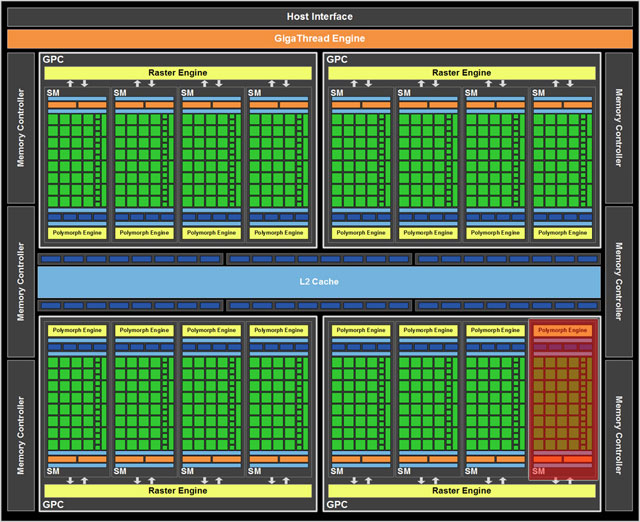
\includegraphics[width=0.7\linewidth]{gtx}
    \caption{NVIDIA GTX480 Architecture}
    \label{fig:gtx}
\end{figure}
\FloatBarrier

\begin{table}[!ht]
\centering
\begin{tabular}{l|l}
Microarchitecture & Fermi \\ \hline
Compute capability (version) & 2.0 \\ \hline
Maximum dimensionality of grid of thread blocks & 3 \\ \hline
Maximum x-dimension of a grid of thread blocks & 65535 \\ \hline
Maximum y-, or z-dimension of a grid of thread blocks & 65535 \\ \hline
Maximum dimensionality of thread block & 3 \\ \hline
Maximum x- or y-dimension of a block & 1024 \\ \hline
Maximum number of threads per block & 1024 \\ \hline
Cores per SM (warp size) & 32 \\ \hline
SM & 15 \\ \hline
Cores & 480 (32 * 15) \\ \hline
Maximum number of resident blocks per multiprocessor & 8 \\ \hline
Maximum number of resident warps per multiprocessor & 48 \\ \hline
Maximum number of resident threads per multiprocessor & 1536 (48 * 32) \\ \hline
Number of 32-bit registers per multiprocessor & 32K \\ \hline
Maximum amount of shared memory per multiprocessor & 48K \\ \hline
Theoretical Throughput & 1345 GFLOPS \\ \hline
Theoretical Bandwidth & 177.4 GB/s
\end{tabular}
\caption{NVIDIA GTX480 Specifications}
\label{table:t1}
\end{table}

\section{CImg}
\label{sec:cimg}
The image processing library used in this project was CImg, a small, modern and open-source toolkit developed for C++. CImg implements the RGB color model, an additive color model in which red, green, and blue light are added together in various ways to reproduce a broad array of colors. Each colored image of size \textit{N*M} is composed by three parts (R,G,B) of the same size, so that \textit{N*M*3} values are necessary to define an image. The Figure \ref{fig:rgb} shows an example of image composition.

\begin{figure}[!ht]
    \centering
    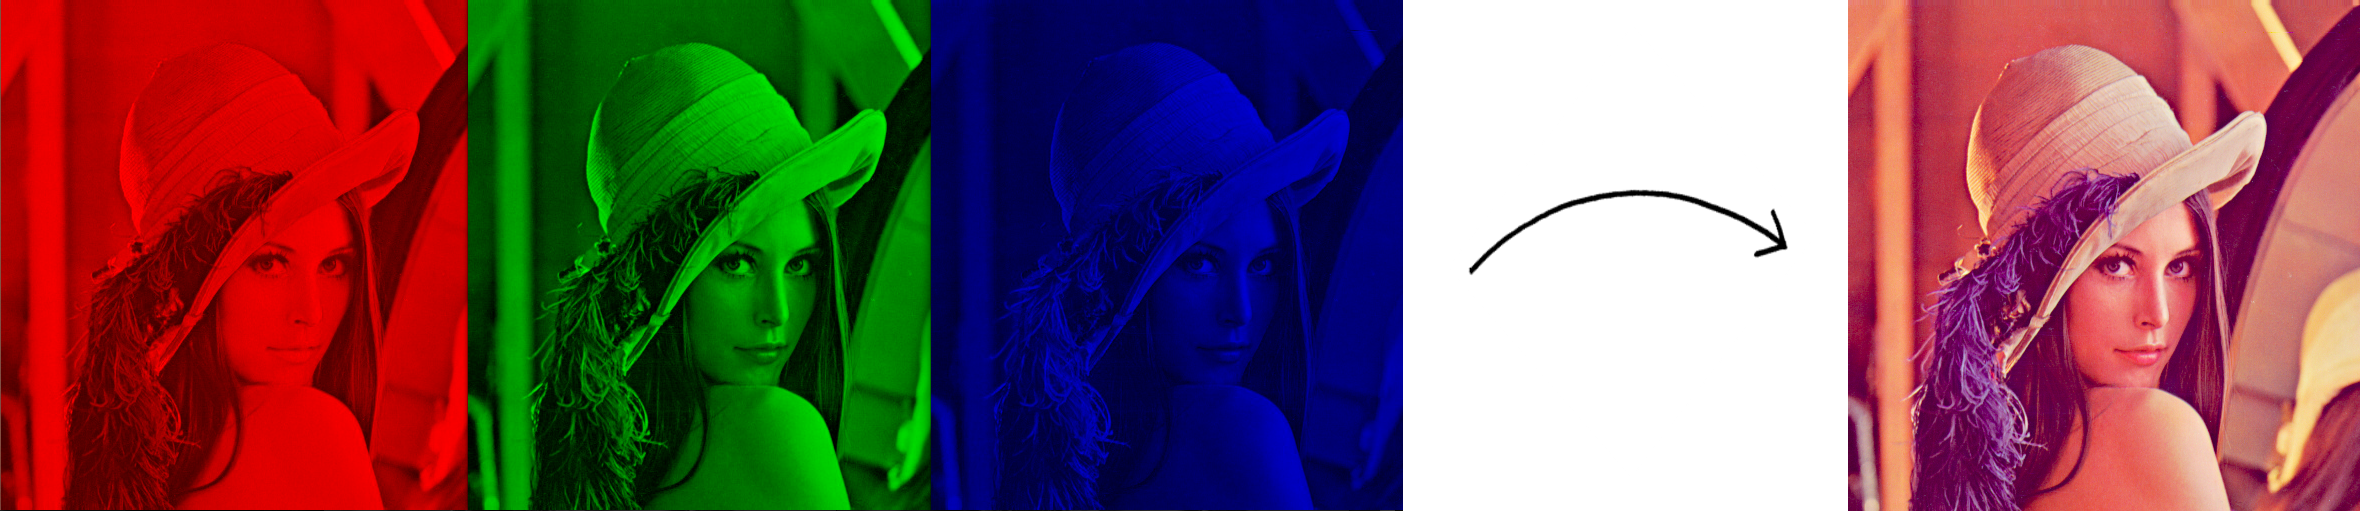
\includegraphics[width=0.7\linewidth]{rgb}
    \caption{RGB model}
    \label{fig:rgb}
\end{figure}
\FloatBarrier

\section{The processing flow}
\label{sec:cpf}
Using CUDA there are two parts of the code: the device code, or GPU code, or the Kernel, that is a sequential program, written for one thread and executed for all and the HOST code, or CPU code, that is used to instantiate the grid, run the kernel, manage the memory. Figure \ref{fig:flow} shows the processing flow of a CUDA application. In the particular case of image processing, everything starts from the CPU, that stores the image from a file into a local buffer, allocates IN and OUT buffers on the GPU (\textit{cudaMalloc}) and copies the image into the GPU's IN buffer (\textit{cudaMemCpy}). After that, the CPU launches the GPU kernel with a defined grid configuration (\textit{kernel\_function <<gridDim, blockDim>>(params)}), that is executed by the GPU following the SIMT (Single Instruction, Multiple Threads) NVIDIA model. The threads are executed in parallel in each core, and they read the assigned part of IN data and generates the assigned part of OUT data. At the end, the results are copied out back to the CPU (\textit{cudaMemCpy}) and the image is written to a file by the CPU.

\begin{figure}[!ht]
    \centering
    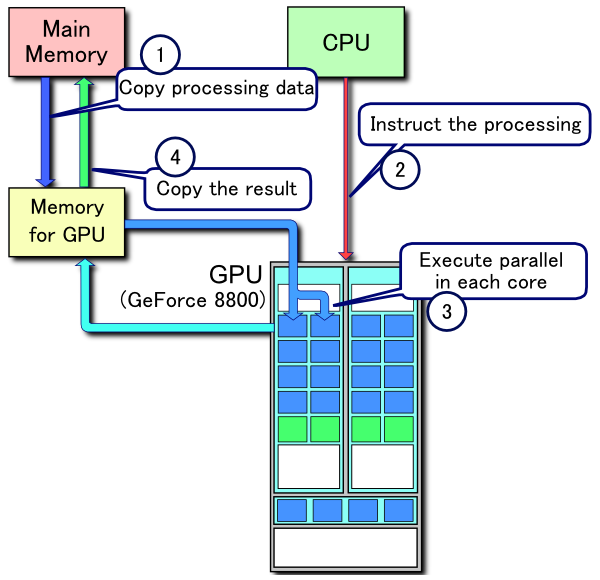
\includegraphics[width=0.5\linewidth]{flow}
    \caption{CUDA processing flow}
    \label{fig:flow}
\end{figure}
\FloatBarrier

\section{CUDA grid configuration}
\label{sec:grid}
In CUDA, as mentioned before, there is a strinct mapping with the hardware, so that an hardware virtualization model is fixed with the concepts of thread, block and grid.
Each \textbf{thread} executes the kernel code, running on one CUDA core.
The threads are logically grouped into \textbf{thread blocks}, so that the threads of the same block will run on the same multiprocessor. The thread blocks are logically organized in a \textbf{Grid}, that represent the entire dataset. The blocks and the grid can be of 1D, 2D or 3D.
The most important thing programming with GPUs, to make use of all their power, is to make them as busy as possible. Switching between concurrent warps has no overhead because registers and share memory are partitioned and not stored/restored, so that if one warp has to wait for example for a memory access and another warp is ready, there is a switch to hide the latency. The thread scheduling is really quick, and this allow the blocks to be swapped in and out really quickly. For this reason an high number of warps is needed and instantiating a grid, is good to have a number of blocks much bigger than the number of available multiprocessor and a block size that can be higher than the amount of cuda cores available per SM.
Another interesting aspect to take into consideration, is the block size. The block is divided into warps, so that Threads 0..31 are part of Warp 0, Threads 32...63 are part of Warp 1 and so on. Considering this, it is good to have blocks with a size multiple of 32, so that no useless threads are launched. For what concerning the grid configuration, an image is a 2D structure and for this reason it is intuitive to set up also a 2D grid. By the way, setting up a 2D grid, there is not only one way to follow. For this particular project three possible block configurations were considered, 1D (1x256), 2D (8x32), 2D (16x32) and two possible grid configurations: dynamic and fixed. In the rest part of this document, for dynamic grid configurations, \textbf{M1} indicates a dynamic grid of 1D blocks, in which the grid has a height of \textit{image\_height}, a width of \textit{(ceil(image\_width / 256))} and the threads on the right border if the image width is not a multiple of \textit{block\_width} are idle (Figure \ref{fig:m1}); \textbf{M2} indicates a dynamic grid of 1D blocks, in which the size of the grid is the same as M1, but the threads are consecutive and only the threads on the last block(s) are idle if the image's number of pixel is not a multiple of the size of the block (Figure \ref{fig:m2}); \textbf{M3} indicates a dynamic grid of 2D blocks, in which the grid has a width of \textit{ceil(image\_width / 32)}, a height of \textit{ceil(image\_height / 8)} and the overflow is the same as M1 (Figure \ref{fig:m3}); \textbf{M4} indicates a dynamic grid of 2D blocks, in which the size of the grid is the same as M3, but the oveflow is the same as M2 (Figure \ref{fig:m4}). The advantages using a fixed grid configuration are that it is possible to support any problem size even if it exceeds the largest grid size the CUDA device supports and that it is possible to limit the number of blocks, for example launching a number of blocks that is a multiple of the number of multiprocessors on the device, to balance utilization.

\begin{figure}[!ht]
\begin{subfigure}{0.5\textwidth}
\centering
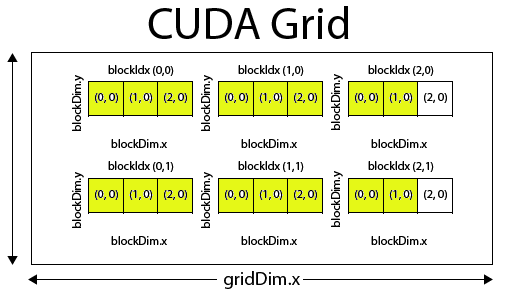
\includegraphics[width=\linewidth]{res/M1}
\caption{M1 - Right overflow}
\label{fig:m1}
\end{subfigure} % separation between the subfigures
\begin{subfigure}{0.5\textwidth}
\centering
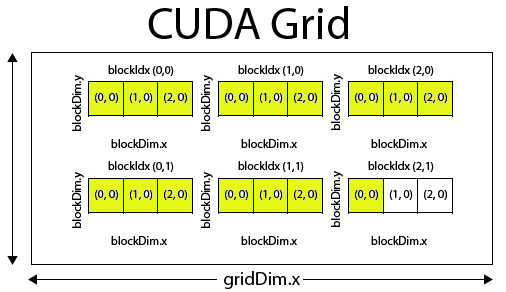
\includegraphics[width=\linewidth]{res/M2}
\caption{M2 - Overflow at the end}
\label{fig:m2}
\end{subfigure}
\caption{1D blocks, Kernel configurations, image of 16 pixels}
 \label{fig:methods12}
\end{figure}
\FloatBarrier

\begin{figure}[!ht]
 % separation between the subfigures
\begin{subfigure}{0.5\textwidth}
\centering
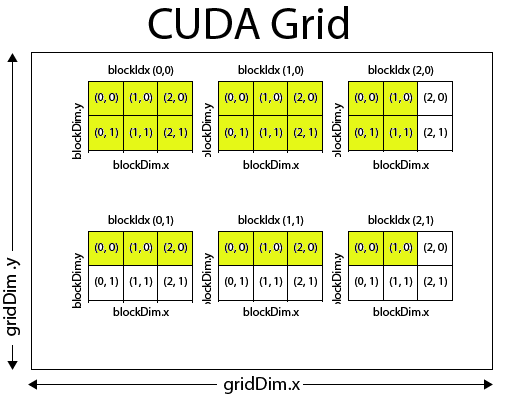
\includegraphics[width=\linewidth]{res/M3}
\caption{M3 - Right overflow}
\label{fig:m3}
\end{subfigure}
 % separation between the subfigures
\begin{subfigure}{0.5\textwidth}
\centering
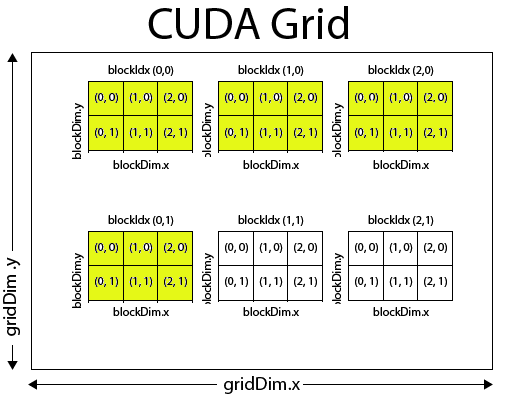
\includegraphics[width=\linewidth]{res/M4}
\caption{M4 - overflow at the end}
\label{fig:m4}
\end{subfigure}
\caption{2D blocks possible kernel configurations, image of 24 pixels}
 \label{fig:methods34}
\end{figure}
\FloatBarrier

\section{Coalesced memory access}
\label{sec:cma}
One of the main bottlenecks with the GPUs are the global memory accesses that are expensive, for this reason it is better to maximize the use of bytes that travel from the DRAM to the Streaming Multiprocessor. CUDA uses a SIMT approach, in which all threads of a warp execute the same instruction, so that global memory accesses are effectuated "per warp". The threads in a warp (32) provide 32 addresses and the hardware converts these addresses into memory transactions. The memory is divided into regions of 128 bytes, so that bytes 0...127 are part of Region 0, bytes 128...255 are part of Region 1 and so on. The memory is accessed per region, that means if one thread wants the byte 0, the entire Region 0 is loaded. A kernel is correctly designed, if consecutive threads access consecutive memory addresses, so that all the requeted addresses fall on the same region and only one transaction is performed. Behaving in this "coalesced way" instead of having one access per thread, these accesses are grouped and the total memory overhead is reduced. Developing all the three algorithms this aspect was taken into consideration.

\newpage

\section{Algorithm 1: Grayscale Conversion and Darkening}
\label{sec:gcd}
From an RGB image, the output of this algorithm is a darker grayscale image.
The gray value of a pixel is generated by weighting the three values (\texttt{0.3*R, 0.59*G, 0.11*B}) and then summing them together. To darken the obtained grayscale image, the final pixel value is multiplied by a constant (0.6). The Figure \ref{fig:dark} shows an example of the result. The sequential algorithm, simply go through the entire image and computes for each pixel the corresponding value (Listing \ref{dsc}).

\begin{figure}[!ht]
    \centering
    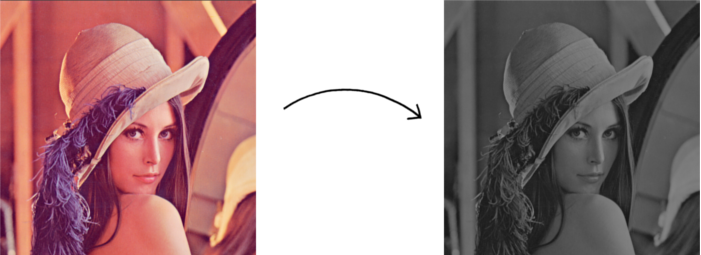
\includegraphics[width=0.7\linewidth]{dark}
    \caption{Grayscale Conversion and Darkening}
    \label{fig:dark}
\end{figure}
\FloatBarrier

\begin{lstlisting}[label=dsc, caption=Darker Sequential code]
//H=image_height, W=image_width
for ( int y = 0; y < H; y++ ) {
 for ( int x = 0; x < W; x++ ) {
  float grayPix = 0.0f;
  float r = static_cast< float >(inputImage[(y * W) + x]);
  float g = static_cast< float >(inputImage[(W * H) + (y * W) + x]);
  float b = static_cast< float >(inputImage[(2 * W * H) + (y * W) + x]);
  grayPix = ((0.3f * r) + (0.59f * g) + (0.11f * b));
  grayPix = (grayPix * 0.6f) + 0.5f;
  darkGrayImage[(y * W) + x] = static_cast< unsigned char >(grayPix);
 }
}
\end{lstlisting}
\FloatBarrier

\subsection{Parallelization}
\label{sec:p1}
\subsection{{One pixel per thread}}
\label{sec:dfm}
After allocating into the GPU global memory some space to contain the input image (\textit{3 * image\_width * image\_height * sizeof(unsigned char)}), copying the input image there and allocating some memory to content the output image (\textit{image\_width * image\_height * sizeof(unsigned char)}), the kernel is ready to be launched. The GPU code is the same as the code content inside the loop of the sequential version (Listing \ref{dsc}), but instead of using the indexes of the loop to access the image pixels, it uses the index associated with the thread. In this first method, only one pixel is computed per thread. To exploit the coalesced memory access, two consecutive threads computes/accesses the values of two consecutive pixels. The 4 different grid configurations (explained in Section \ref{sec:grid}) were tested for this program, in order to establish the best. In Figure \ref{fig:histo_darker} are reported the obtained results. As shown methods M1 and M2 obtained the best results, so with unidimensional blocks the algorithm achieved better speedups. This is probably due to the fewest amount of operations to calculate the index of the pixel associated with each thread, because in this particular task there is no clear advantage on using 1D blocks instead of 2D blocks.
\begin{figure}[!ht]
    \centering
    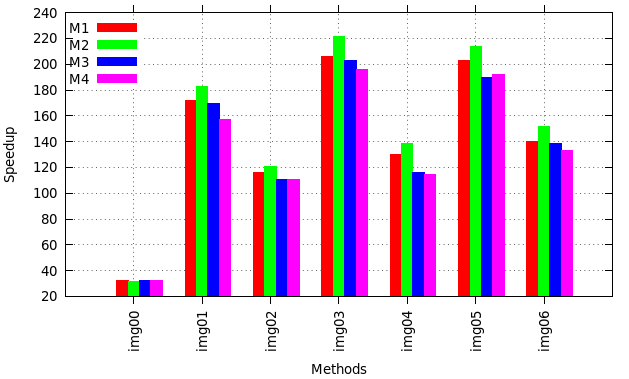
\includegraphics[width=0.9\linewidth]{res/new/darker_confronto}
    \caption{Speedups Comparison}
    \label{fig:histo_darker}
\end{figure}
\FloatBarrier


\subsection{Optimization - More pixels per thread}
\label{sec:dfm}
To exploit all the power of GPUs, as said, they have to be as busy as possible, because the warp scheduling is very fast and can hide the latency. Anyway, reducing the number of thread blocks by increasing the work per thread revealed to achieve better results. Lots of experiments were performed to establish the right number of pixels to compute by each thread, all taking into account the coalesced memory access. To maintain the coalescing, one thread computes the associated first pixel index with the formula shown in Listing \ref{cfp} and then for the following pixels, it adds each time to this the total amount of pixels contained in the grid(\textit{gridDim.x * blockDim.x * gridDim.y * blockDim.y}). The final code, is the one shown in Listing \ref{dpc}. 

\begin{lstlisting}[label=cfp, caption=Corresponding first pixel]
unsigned int pixel=((blockIdx.y * gridDim.x + blockIdx.x) 
                   * blockDim.x) + threadIdx.x
\end{lstlisting}
\FloatBarrier

\begin{lstlisting}[label=dpc, caption=Darker Parallel Code]
for(i = ((blockIdx.y * gridDim.x + blockIdx.x) * blockDim.x) + threadIdx.x; 
    i < width * height; 
    i += (gridDim.x * blockDim.x) * (gridDim.y * blockDim.y)) {
  float grayPix = 0.0f;
  float r = static_cast< float >(inputImage[i]);
  float g = static_cast< float >(inputImage[(width * height) + i]);
  float b = static_cast< float >(inputImage[(2 * width * height) + i]);
  grayPix = ((0.3f * r) + (0.59f * g) + (0.11f * b));
  grayPix = (grayPix * 0.6f) + 0.5f;
  outputDarkGrayImage[i] = static_cast< unsigned char >(grayPix);
}
\end{lstlisting}
\FloatBarrier

Figures \ref{fig:darker_try_histo} and \ref{fig:darker_fixed} represent the speedups achieved for different thread loads, considering both a dynamic and a fixed grid. Figure \ref{fig:compare_darker} compares the best results for the two configurations. As it is possible to see, the first approach achieved better results. With a number of 10 pixels per thread, the program obtained the best results, so this is a good thread load to help the scheduler. This load was sufficient to both hide the latency and reduce the warp scheduling overhead. Figure \ref{fig:darker_single_more_comparison} shows the comparison between the best results obtained with a single pixel per thread and the results obtained with the new version. It is clear that the new version is an optimization, in fact for each image the speedup increased. This solution is the one adopted. In Table \ref{tab:darker_ex} and \ref{tab:darker_sp} are shown the detailed execution times and speedups achieved. Table \ref{dmt} shows the total time considering also the memory overhead. Table \ref{tab:darker_t_b} exposes the Achieved Throughput and Bandwidth. For the Throughput, for each pixel there are 3 additions and 4 multiplications. For the Bandwidth, for each pixel there are 3 reads and 1 write of 1 byte.  Table \ref{tab:pxabd} exposes the differences obtained comparing the output of the sequential algorithm with the output of the parallel algorithm. These differences could derive from a difference in floating point precision between the CPU and GPU, or from different ordering of floating point operations. In Section \ref{sec:vp} is reported a detailed analysis using the NVIDIA Virtual Profiler.
    
\begin{figure}[!ht]
    \centering
    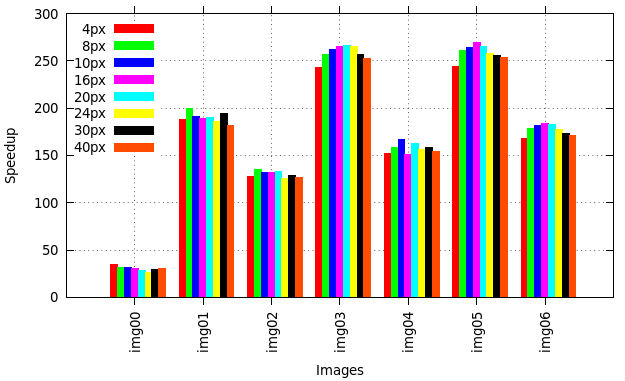
\includegraphics[width=0.8\linewidth]{res/new/darker_try_histo}
    \caption{Speedup with different number of pixels per thread}
    \label{fig:darker_try_histo}
\end{figure}
\FloatBarrier

\begin{figure}[!ht]
    \centering
    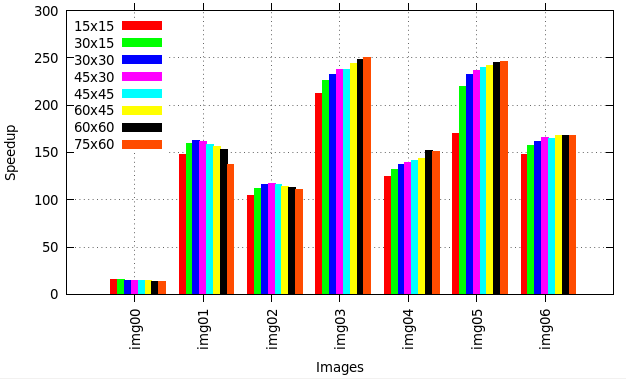
\includegraphics[width=0.8\linewidth]{res/new/darker_fixed}
    \caption{Speedup with fixed grid}
    \label{fig:darker_fixed}
\end{figure}
\FloatBarrier

\begin{figure}[!ht]
    \centering
    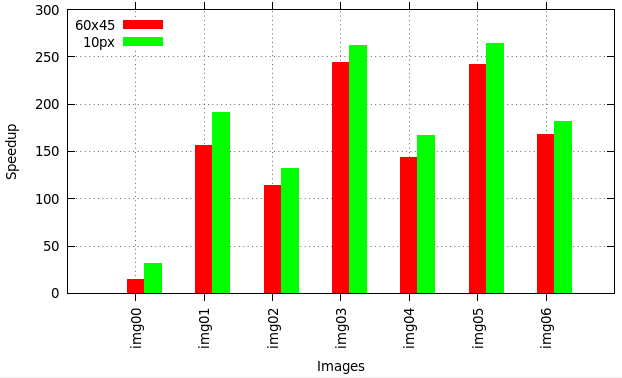
\includegraphics[width=0.7\linewidth]{res/new/darker_best_compare}
    \caption{Solutions Comparison}
    \label{fig:compare_darker}
\end{figure}
\FloatBarrier

\begin{figure}[!ht]
    \centering
    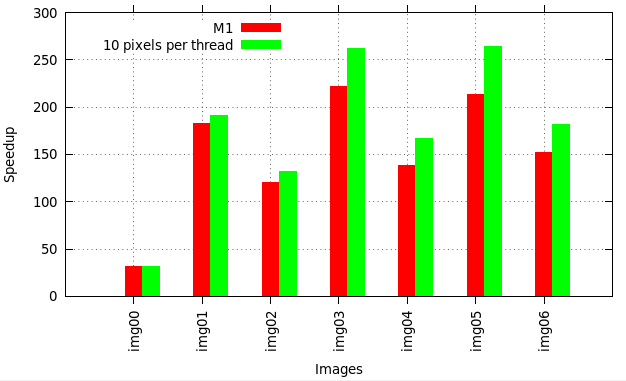
\includegraphics[width=0.7\linewidth]{res/new/darker_single_more_comparison}
    \caption{Solutions comparison}
    \label{fig:darker_single_more_comparison}
\end{figure}
\FloatBarrier

\begin{table}[!ht]
\centering
\begin{tabular}{|c|l|c|c|}
\hline
               & \textbf{Sequential} & \textbf{M2} & \textbf{10 pixels per thread} \\ \hline
\textbf{img00} & 0.002416            & 0.000076    & 0,000076                      \\ \hline
\textbf{img01} & 0.036925            & 0.000202    & 0,000193                      \\ \hline
\textbf{img02} & 0.033726            & 0.000279    & 0,000255                      \\ \hline
\textbf{img03} & 0.340821            & 0.001537    & 0,001299                      \\ \hline
\textbf{img04} & 0.151429            & 0.001091    & 0,000907                      \\ \hline
\textbf{img05} & 0.445976            & 0.002090    & 0,001692                      \\ \hline
\textbf{img06} & 0.588814            & 0.003880    & 0,003239                      \\ \hline
\end{tabular}
\caption{Execution Times}
\label{tab:darker_ex}
\end{table}
\FloatBarrier

\begin{table}[!ht]
\centering
\begin{tabular}{|c|c|c|}
\hline
               & \textbf{M2} & \textbf{10 pixels per thread} \\ \hline
\textbf{img00} & 31.79       & 31.79                         \\ \hline
\textbf{img01} & 182.80      & 191.32                        \\ \hline
\textbf{img02} & 120.88      & 132.26                        \\ \hline
\textbf{img03} & 221.74      & 262.37                        \\ \hline
\textbf{img04} & 138.80      & 166.96                        \\ \hline
\textbf{img05} & 213.39      & 263.58                        \\ \hline
\textbf{img06} & 151.76      & 181.79                        \\ \hline
\end{tabular}
\caption{Speedups}
\label{tab:darker_sp}
\end{table}
\FloatBarrier


\begin{table}[!ht]
\centering
\begin{tabular}{|l|c|c|c|}
\hline
\textbf{Images} & \textbf{Execution Time (s)} & \textbf{Memory Time(s)} & \textbf{Total(s)} \\ \hline
\textbf{Img00}  & 0,000076                    & 0,000547                & 0,077502          \\ \hline
\textbf{Img01}  & 0,000193                    & 0,004562                & 0,081866          \\ \hline
\textbf{Img02}  & 0,000255                    & 0,006141                & 0,072205          \\ \hline
\textbf{Img03}  & 0,001299                    & 0,031491                & 0,108873          \\ \hline
\textbf{Img04}  & 0,000907                    & 0,025354                & 0,103170          \\ \hline
\textbf{Img05}  & 0,001692                    & 0,049163                & 0,125342          \\ \hline
\textbf{Img06}  & 0,003239                    & 0,079937                & 0,158472          \\ \hline
\end{tabular}
\caption{Measured times}
\label{dmt}
\end{table}
\FloatBarrier




\begin{table}[!ht]
\centering
\begin{tabular}{|c|c|c|c|c|}
\hline
               & \textbf{\begin{tabular}[c]{@{}c@{}}Ach. Throughput\\ (GFLOPS/s)\end{tabular}} & \textbf{\begin{tabular}[c]{@{}c@{}}Ach. Bandwidth \\ (GB/s)\end{tabular}} & \textbf{\begin{tabular}[c]{@{}c@{}}Compute utilization \\ (\%)\end{tabular}} & \textbf{\begin{tabular}[c]{@{}c@{}}Bandwidth utilization \\ (\%)\end{tabular}} \\ \hline
\textbf{Img00} & 24,14                                                                             & 13,80                                                                         & 1,80                                                                         & 7,78                                                                           \\ \hline
\textbf{Img01} & 95,08                                                                             & 54,33                                                                         & 7,07                                                                         & 30,63                                                                          \\ \hline
\textbf{Img02} & 101,20                                                                            & 57,83                                                                         & 7,52                                                                         & 32,60                                                                          \\ \hline
\textbf{Img03} & 136,02                                                                            & 77,72                                                                         & 10,11                                                                        & 43,81                                                                          \\ \hline
\textbf{Img04} & 129,48                                                                            & 73,99                                                                         & 9,63                                                                         & 41,71                                                                          \\ \hline
\textbf{Img05} & 137,11                                                                            & 78,35                                                                         & 10,19                                                                        & 44,16                                                                          \\ \hline
\textbf{Img06} & 141,63                                                                            & 80,93                                                                         & 10,53                                                                        & 45,62                                                                          \\ \hline
\end{tabular}
\caption{Achieved Throughput and Bandwidth}
\label{tab:darker_t_b}
\end{table}
\FloatBarrier

\begin{table}[!ht]
\centering
\begin{tabular}{|c|l|c|c|l|l|l|l|}
\hline
\textbf{}                        & \textbf{img00}           & \textbf{img01} & \textbf{img02} & \textbf{img03}           & \textbf{img04}            & \textbf{img05}         & \textbf{img06}            \\ \hline
\textbf{Pixels above  threshold} & \multicolumn{1}{c|}{111} & 231            & 135            & \multicolumn{1}{c|}{735} & \multicolumn{1}{c|}{1503} & \multicolumn{1}{c|}{9} & \multicolumn{1}{c|}{4206} \\ \hline
\end{tabular}
\caption{Differences between the Sequential and the Parallel output}
\label{tab:pxabd}
\end{table}
\FloatBarrier

\newpage

\section{Algorithm 2: Histogram Computation}
\label{sec:hc}
From an RGB image, the output of this algorithm is a grayscale image with the relative histogram of 256 possible values of gray.
The histogram measures how often a value of gray is used in an image. The sequential algorithm, simply go through the entire image, computing for each pixel the corresponding gray value and incrementing the corresponding counter (Listing \ref{histo_loop}). The Figure \ref{fig:histo} shows an example of the result.

\begin{lstlisting}[label=histo_loop, caption=Sequential code]
//H=image_height , W=image_width
for ( int y = 0; y < H; y++ ) {
 for ( int x = 0; x < W; x++ ) {
  float grayPix = 0.0f;
  float r = static_cast< float >(inputImage[(y * W) + x]);
  float g = static_cast< float >(inputImage[(W * H) + (y * W) + x]);
  float b = static_cast< float >(inputImage[(2 * W * H) + (y * W) + x]);
  grayPix = ((0.3f * r) + (0.59f * g) + (0.11f * b)) + 0.5f;
  grayImage[(y * W) + x] = static_cast< unsigned char >(grayPix);
  histogram[static_cast< unsigned int >(grayPix)] += 1;
 }
}
\end{lstlisting}

\begin{figure}[!ht]
    \centering
    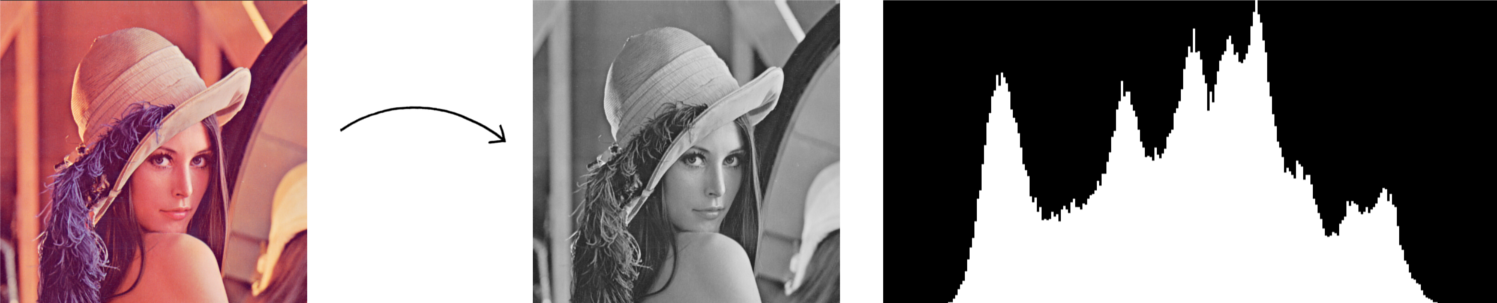
\includegraphics[width=0.7\linewidth]{histo}
    \caption{Histogram Computation}
    \label{fig:histo}
\end{figure}
\FloatBarrier

\subsection{Parallelization}
\label{sec:p2}
\subsection{One pixel per thread}
\label{sec:fm2}
After copying the input image (\textit{3 * image\_width * image\_height * sizeof(unsigned char)}) and the initial empty histogram (\textit{256 * sizeof(unsigned int)}) into the GPU global memory and allocating some memory to content the output image (\textit{image\_width * image\_height * sizeof(unsigned char)}), the kernel is ready to be launched. As for the previous algorithm, the GPU code is almost the same as the code content inside the loop of the sequential version (Listing \ref{histo_loop}), but instead of using the indexes of the loop to access the image pixels, it uses the index associated with the thread. Also in this case, to exploit the coalesced memory access, two consecutive threads computes/accesses the values of two consecutive pixels. The interesting aspect of computing histograms in parallel, is that it is possible that two threads read at the same time the same value of gray for a pixel, so that at the same time they try to increment the corresponding histogram bin. For a correct execution, to avoid wrong updates, the increment has to be an atomic operation, so that only one thread at the time will modify the bin value. 
The logic behind an atomic operation is that each thread "locks" the variable, modify it, and "unlocks" it, so that the other threads that try to modify the same variable has to wait that this will be "unlocked". The worst case, in the histogram scenario, is a monochrome image (only one color), in which all the threads try to modify the same bin, which implies a long waiting queue of threads. The general idea to have high performance, is to reduce the number of conflicts at the minimum. Also in this algorithm, the speedup is not related to the shape of the block, in fact the performance of the algorithm using the atomics depends on the image. Dealing with an image with horizontal stripes of different colors of 1 pixel, for example, with a 1D block (1x256) there will be all the 256 threads that try to increment the same histogram bin. In the same scenario, using a 2D block (8x32) there will be only 32 threads that try to increment the same histogram value. If the image instead, is composed of vertical stripes of 32 pixels wide, it happens the opposite, the 1D approach will obtain more performance. For these reasons, for the initial tests, to remove the fortuity, the given images were substituted with images of the same sizes but composed by only one color (monochrome). Different implementations were tested. The first approach consisted of using only the histogram array stored in the global memory and modifying it with atomic add operations (Figure \ref{fig:ghgh}). The second approach consisted of using an additional histogram array stored in shared memory, performing the atomic add operations there and at the end, assigning a certain bin to a thread and reducing the shared histograms in the global one (Figure \ref{fig:shsh}). Doing this, not all the launched threads will compete for the same bin, but only the threads in the same block during the computation and the threads to which is assigned the same bin during the reduction phase. Figure \ref{fig:gavsa} shows the obtained results for the two approaches. From this image it is clear that the second approach drastically increased the speedups and that the block configuration (1D or 2D) doesn't affect the performance.

\begin{figure}[!ht]
    \centering
    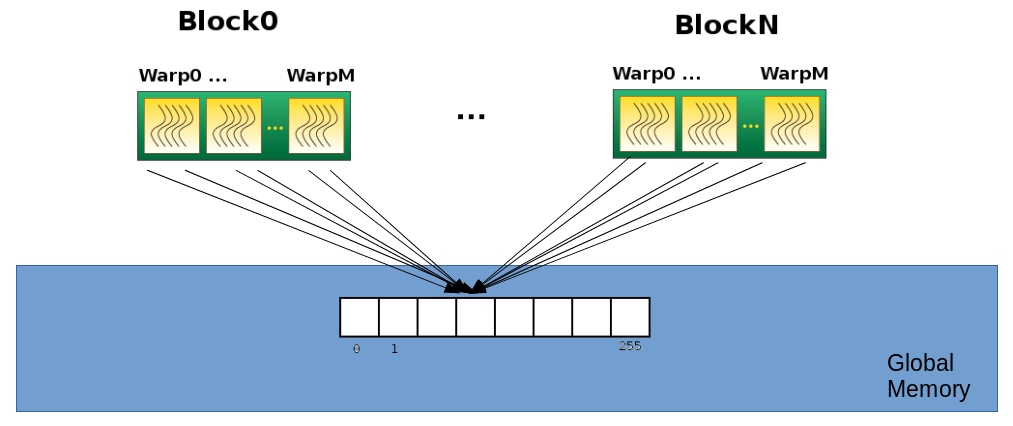
\includegraphics[width=0.7\linewidth]{global_histo}
    \caption{Global histogram - Concurrency}
    \label{fig:ghgh}
\end{figure}
\FloatBarrier

\begin{figure}[!ht]
    \centering
    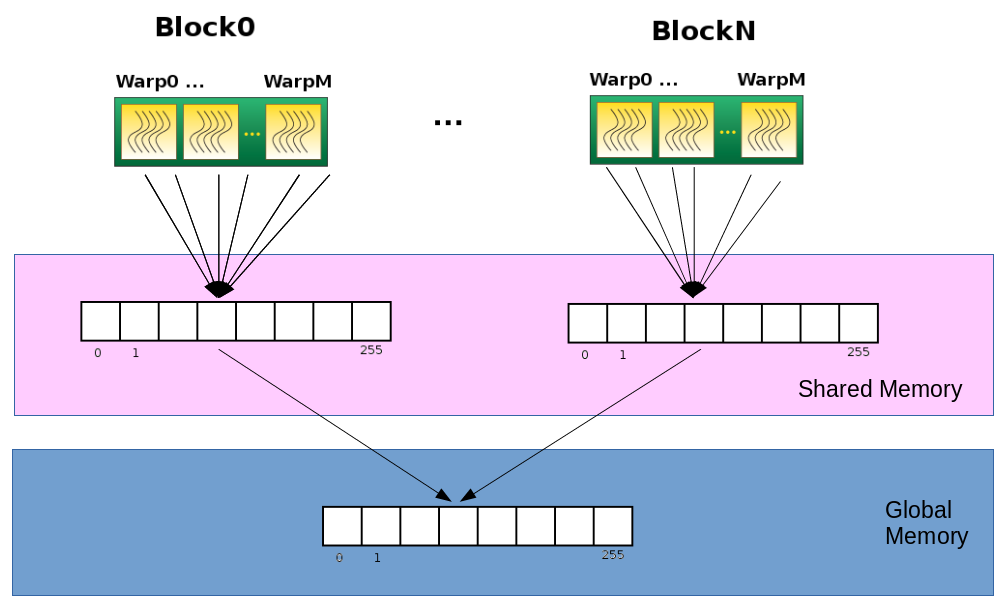
\includegraphics[width=0.7\linewidth]{shared_histo}
    \caption{Shared histogram - Concurrency}
    \label{fig:shsh}
\end{figure}
\FloatBarrier

\begin{figure}[!ht]
    \centering
    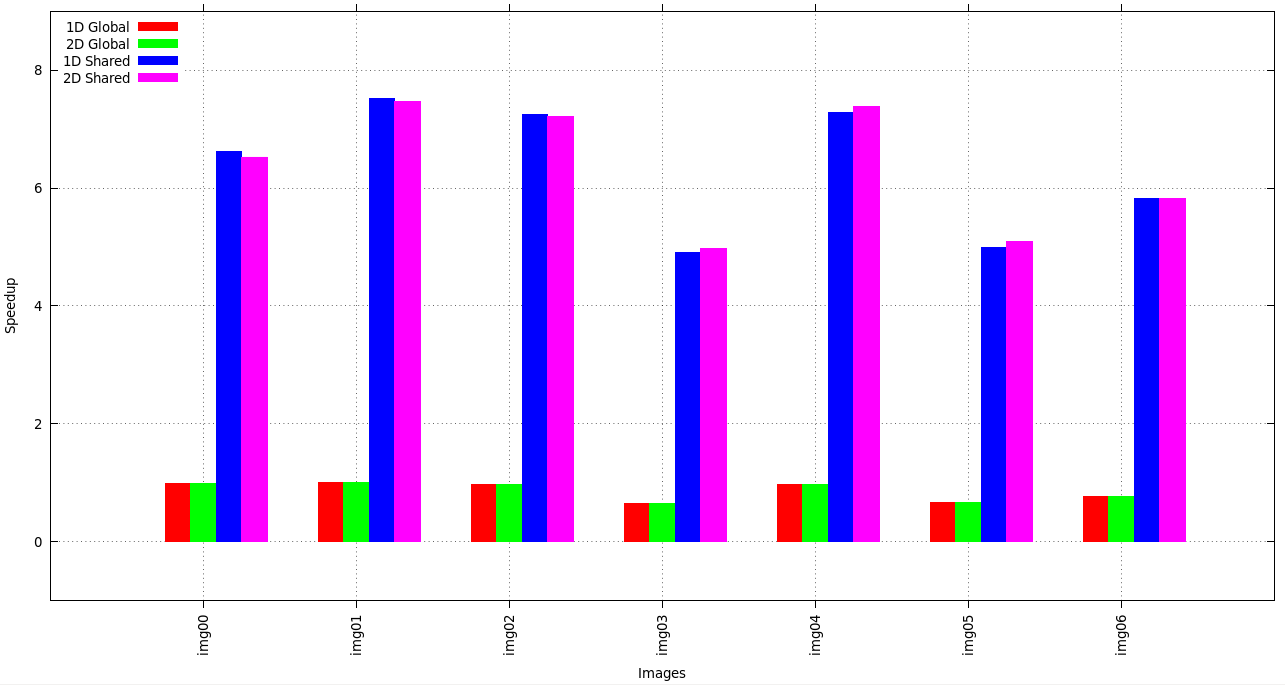
\includegraphics[width=0.7\linewidth]{res/new/histogram_confronto}
    \caption{Global Atomics vs Shared Atomics (Monochrome images)}
    \label{fig:gavsa}
\end{figure}
\FloatBarrier

An additional "privatization" of the histogram could be performed. Instead of having one histogram per block, it is possible to assign one histogram per warp (Figure \ref{fig:whwh}), so that the concurrency at the end is only among the 32 warp threads during the computation and between the threads to which is assigned the same bin during the reducing phase. Figure \ref{fig:sawvsa} shows the performance of this last method compared to the previous. The number of concurrent histogram modifications was reduced, so that better speedups were achieved.

\begin{figure}[!ht]
    \centering
    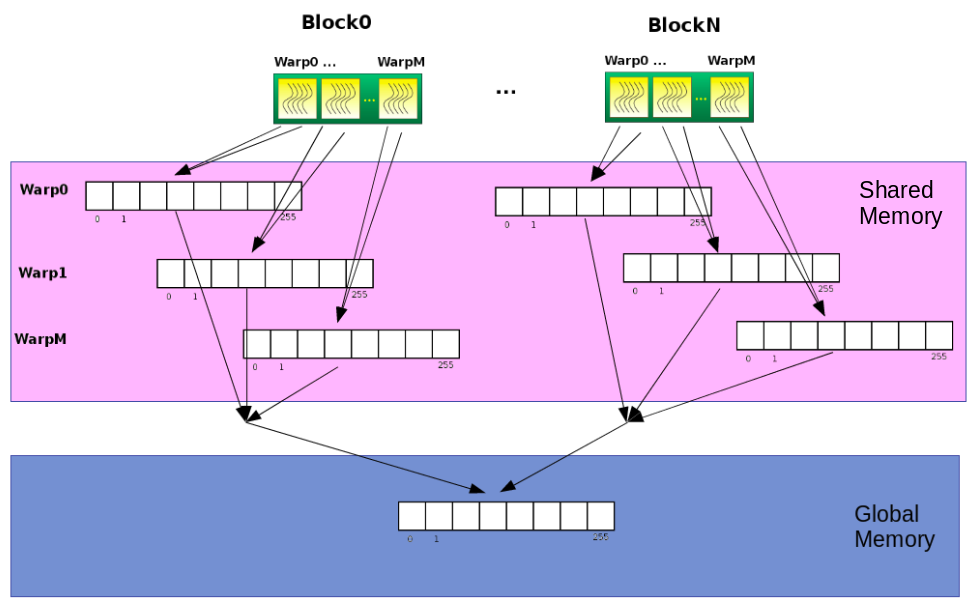
\includegraphics[width=0.9\linewidth]{histo_warp}
    \caption{Shared Warps histogram - Concurrency}
    \label{fig:whwh}
\end{figure}
\FloatBarrier

\begin{figure}[!ht]
    \centering
    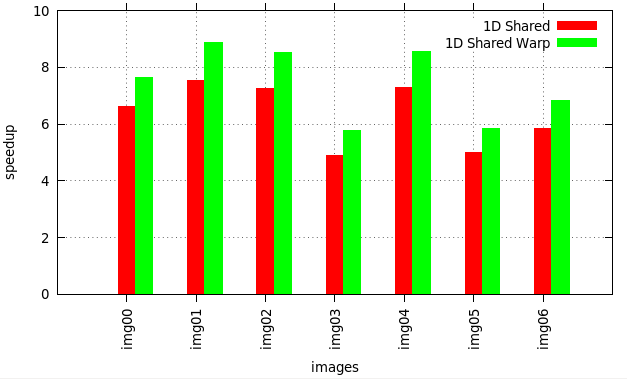
\includegraphics[width=0.7\linewidth]{res/new/histogram_warp}
    \caption{Shared Atomics with Warps vs Shared Atomics (Monochrome images)}
    \label{fig:sawvsa}
\end{figure}
\FloatBarrier

After a testing phase with monochrome images, the tests were performed with the real given images. Figure \ref{fig:gasawvsa} represents the obtained results. As it is possible to see, in this case the warp solution is much worse than the shared version, that means for standard images, the time spent to reduce the single warp histograms is bigger than the time spent to compute the atomic operations. 

\begin{figure}[!ht]
    \centering
    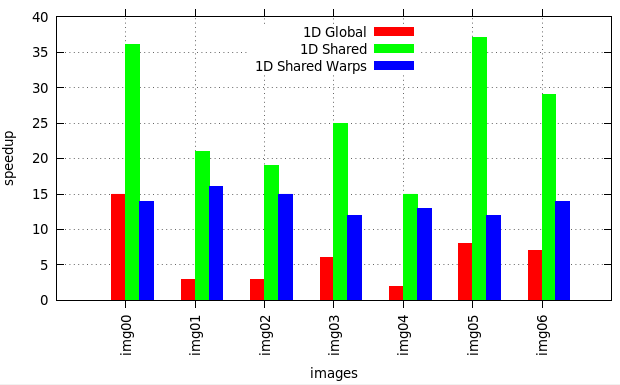
\includegraphics[width=0.7\linewidth]{res/new/histogram_confronto_real}
    \caption{Global Atomics vs Shared Atomics vs Shared Atomics with Warps}
    \label{fig:gasawvsa}
\end{figure}
\FloatBarrier

\subsection{Optimization - More pixels per thread}
\label{sec:hop}
As for the previous algorithm, some additional tests were performed assigning the computation of more pixels per thread. The last two approaches (Shared Atomics and Shared Atomics with Warps) were improved to test this solution and both on the real images obtained better results. This is due to the reduction of the scheduling load and to the decrease of histograms reduction operations. Different work loads were assigned to each thread and measured. A dynamic grid and fixed grid configurations were tested and Figures \ref{fig:hum}, \ref{fig:hfm}, \ref{fig:hwm} and \ref{fig:hwf} show the obtained results. Figure \ref{fig:dbsc} compares the best obtained configurations for the two approaches. As shown, the second approach (Shared Atomics with Warps), differently than the one pixel per thread version, obtains for almost all the images the best results. This result could surprise, but means that the decrement on the total number of reduction operations is critical for this approach. For the small images (e.g. Img00) the time spent for the final reduction remains high in comparison with the total computation due to the low amount of pixels to compute. The final adopted solution is the Shared Atomics with Warps with with a fixed grid, because obtained better results for almost all the images and it is a more scalable solution. Tables \ref{tab:histo_exe} and \ref{tab:histo_sp} show the detailed obtained results. Table \ref{tab:histo_me} shows the total time of the adopted solution, considering also the memory overhead. Table \ref{tab:histo_mtb} exposes the Achieved Throughput and Bandwidth. For the Throughput, for each pixel there are 3 additions, 3 multiplications and 1 shared memory atomic add operation and for each block there are 256*8 additions (warps histogram reduction) and 256 global memory atomic add operations. For the Bandwidth, for each pixel there are 3 reads and 1 write (of 1 byte) and for each block there are 256 writes (of 4 bytes) for the atomic add operations.
Tables \ref{tab:pxabh} and \ref{tab:pxabhg} show the differences obtained comparing the outputs of the sequential algorithm with the outputs of the parallel algorithm.


\begin{figure}[!ht]
    \centering
    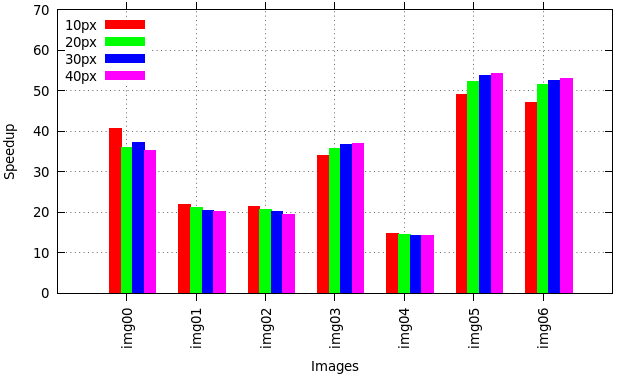
\includegraphics[width=0.65\linewidth]{res/new/histogram_uni_more}
    \caption{Shared Atomics, 1D blocks - Different number of assigned pixels per thread}
    \label{fig:hum}
\end{figure}
\FloatBarrier

\begin{figure}[!ht]
    \centering
    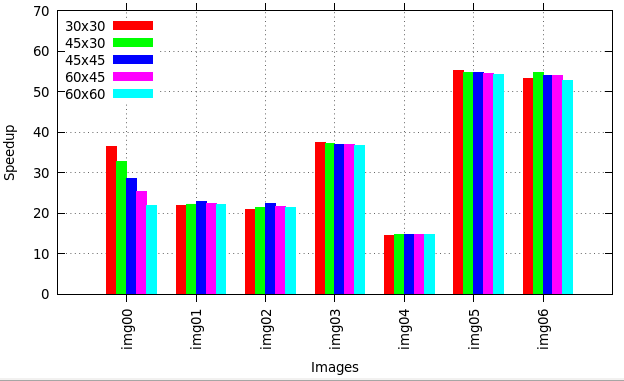
\includegraphics[width=0.65\linewidth]{res/new/histogram_uni_fixed}
    \caption{Shared Atomics, 1D blocks - Fixed grid}
    \label{fig:hfm}
\end{figure}
\FloatBarrier

\begin{figure}[!ht]
    \centering
    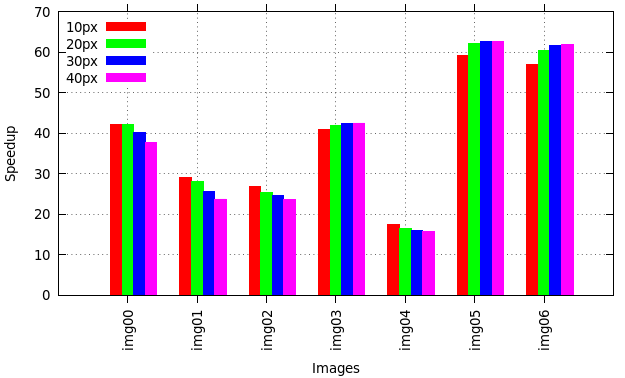
\includegraphics[width=0.65\linewidth]{res/new/histogram_warp_more}
    \caption{Shared Atomics with Warps, 1D blocks - Different number of assigned pixels per thread}
    \label{fig:hwm}
\end{figure}
\FloatBarrier

\begin{figure}[!ht]
    \centering
    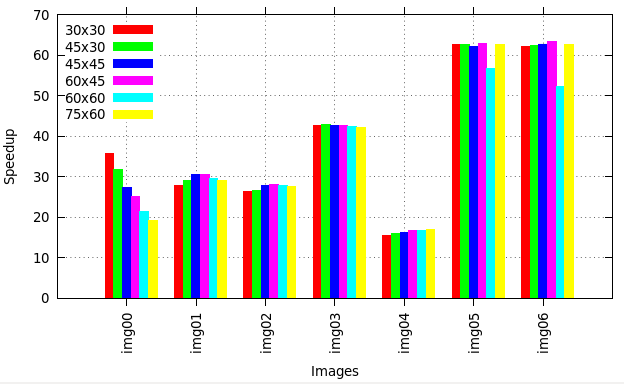
\includegraphics[width=0.7\linewidth]{res/new/histogram_warp_fixed}
    \caption{Shared Atomics with Warps, 1D blocks - Fixed grid}
    \label{fig:hwf}
\end{figure}
\FloatBarrier

\begin{figure}[!ht]
    \centering
    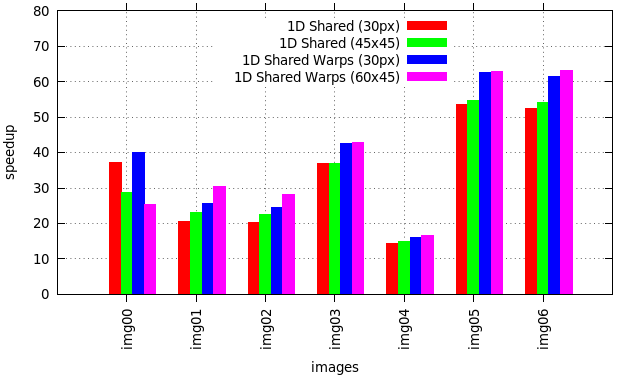
\includegraphics[width=0.7\linewidth]{res/new/histogram_more_confronto}
    \caption{Best solutions comparison}
    \label{fig:dbsc}
\end{figure}
\FloatBarrier

\begin{table}[!ht]
\centering
\begin{tabular}{|l|l|l|l|}
\hline
\multicolumn{1}{|c|}{\textbf{}}      & \textbf{Sequential} & \textbf{30px}                 & \multicolumn{1}{c|}{\textbf{60x45}} \\ \hline
\multicolumn{1}{|c|}{\textbf{Img00}} & 0,003208            & \multicolumn{1}{c|}{0,000080} & \multicolumn{1}{c|}{0,000127}       \\ \hline
\textbf{Img01}                       & 0,032379            & 0,001264                      & 0,001062                            \\ \hline
\textbf{Img02}                       & 0,043784            & 0,001778                      & 0,001553                            \\ \hline
\textbf{Img03}                       & 0,200681            & 0,004724                      & 0,004698                            \\ \hline
\textbf{Img04}                       & 0,197973            & 0,012325                      & 0,011871                            \\ \hline
\textbf{Img05}                       & 0,267590            & 0,004278                      & 0,004260                            \\ \hline
\textbf{Img06}                       & 0,616924            & 0,010026                      & 0,009756                            \\ \hline
\end{tabular}
\caption{Execution Times}
\label{tab:histo_exe}
\end{table}
\FloatBarrier

\begin{table}[!ht]
\centering
\begin{tabular}{|l|l|l|}
\hline
\multicolumn{1}{|c|}{}               & \textbf{30px}              & \multicolumn{1}{c|}{\textbf{60x45}} \\ \hline
\multicolumn{1}{|c|}{\textbf{Img00}} & \multicolumn{1}{c|}{40.10} & \multicolumn{1}{c|}{25.26}          \\ \hline
\textbf{Img01}                       & 25.62                      & 30.49                               \\ \hline
\textbf{Img02}                       & 24.63                      & 28.19                               \\ \hline
\textbf{Img03}                       & 42.48                      & 42.72                               \\ \hline
\textbf{Img04}                       & 16.06                      & 16.68                               \\ \hline
\textbf{Img05}                       & 62.55                      & 62.81                               \\ \hline
\textbf{Img06}                       & 61.53                      & 63.24                               \\ \hline
\end{tabular}
\caption{Speedups}
\label{tab:histo_sp}
\end{table}
\FloatBarrier

\begin{table}[!ht]
\centering
\begin{tabular}{|l|c|c|c|}
\hline
\textbf{Images} & \textbf{Execution Time (s)} & \textbf{Memory Time(s)} & \textbf{Total(s)} \\ \hline
\textbf{Img00}  & 0,000127                    & 0.000645                & 0.070765          \\ \hline
\textbf{Img01}  & 0,001062                    & 0.003966                & 0.070738          \\ \hline
\textbf{Img02}  & 0,001553                    & 0.006266                & 0.073200          \\ \hline
\textbf{Img03}  & 0,004698                    & 0.037846                & 0.118953          \\ \hline
\textbf{Img04}  & 0,011871                    & 0.019135                & 0.096683          \\ \hline
\textbf{Img05}  & 0,004260                    & 0.036651                & 0.105514          \\ \hline
\textbf{Img06}  & 0,009756                    & 0.097466                & 0.182628          \\ \hline
\end{tabular}
\caption{Measured times}
\label{tab:histo_me}
\end{table}
\FloatBarrier

\begin{table}[!ht]
\centering
\begin{tabular}{|l|c|c|c|c|}
\hline
\textbf{Images} & \textbf{\begin{tabular}[c]{@{}c@{}}Ach. Throughput\\ (GFLOPS/s)\end{tabular}} & \textbf{\begin{tabular}[c]{@{}c@{}}Ach. Bandwidth\\ (GB/s)\end{tabular}} & \textbf{\begin{tabular}[c]{@{}c@{}}Compute utilization\\ (\%)\end{tabular}} & \textbf{\begin{tabular}[c]{@{}c@{}}Bandwidth utilization\\ (\%)\end{tabular}} \\ \hline
\textbf{Img00}  & 63,43                                                                         & 30,03                                                                    & 4,72                                                                        & 16,93                                                                         \\ \hline
\textbf{Img01}  & 23,14                                                                         & 12,48                                                                    & 1,72                                                                        & 7,03                                                                          \\ \hline
\textbf{Img02}  & 20,62                                                                         & 11,28                                                                    & 1,53                                                                        & 6,36                                                                          \\ \hline
\textbf{Img03}  & 38,93                                                                         & 22,08                                                                    & 2,89                                                                        & 12,45                                                                         \\ \hline
\textbf{Img04}  & 10,42                                                                         & 5,89                                                                     & 0,77                                                                        & 3,32                                                                          \\ \hline
\textbf{Img05}  & 55,92                                                                         & 31,77                                                                    & 4,16                                                                        & 17,91                                                                         \\ \hline
\textbf{Img06}  & 47,66                                                                         & 27,15                                                                    & 3,54                                                                        & 15,31                                                                         \\ \hline
\end{tabular}
\caption{Achieved Throughput and Bandwidth}
\label{tab:histo_mtb}
\end{table}
\FloatBarrier


\begin{table}[!ht]
\centering
\begin{tabular}{|c|l|c|c|l|l|l|l|}
\hline
\textbf{}                        & \textbf{img00}           & \textbf{img01} & \textbf{img02} & \textbf{img03}          & \textbf{img04}         & \textbf{img05}          & \textbf{img06}          \\ \hline
\textbf{Pixels above  threshold} & \multicolumn{1}{c|}{324} & 12             & 0              & \multicolumn{1}{c|}{24} & \multicolumn{1}{c|}{0} & \multicolumn{1}{c|}{12} & \multicolumn{1}{c|}{48} \\ \hline
\end{tabular}
\caption{Differences between the Sequential and the Parallel output (histogram)}
\label{tab:pxabh}
\end{table}
\FloatBarrier

\begin{table}[!ht]
\centering
\begin{tabular}{|c|c|c|c|c|l|l|l|}
\hline
\textbf{Images}                 & \textbf{Img00} & \textbf{Img01} & \textbf{Img02} & \textbf{Img03} & \textbf{Img04} & \textbf{Img05} & \textbf{Img06} \\ \hline
\textbf{Pixels above threshold} & 777            & 5322           & 849            & 3450           & 8004           & 1431           & 28956          \\ \hline
\end{tabular}
\caption{Differences between the Sequential and the Parallel output (gray image)}
\label{tab:pxabhg}
\end{table}
\FloatBarrier
 
\section{Algorithm 3: Smoothing}
\label{sec:smoo}
Smoothing is the process of removing noise from an image by the means of statistical analysis. To remove the noise, each point is replaced by a weighted average of its neighbours. In this way small-scale structures are removed from the image. In this case a two-dimensional 5-points triangular smooth filter was used. The Figure \ref{fig:smooth} shows an example of the result.

\begin{figure}[!ht]
    \centering
    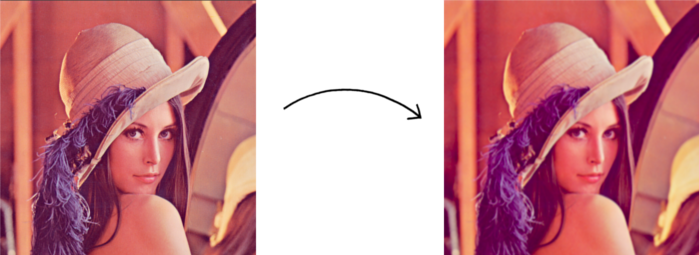
\includegraphics[width=0.5\linewidth]{smooth}
    \caption{Smoothing}
    \label{fig:smooth}
\end{figure}
\FloatBarrier


\subsection{Parallelization}
\label{sec:p3}
\subsection{One pixel per thread}
\label{sec:opts}
After copying the input image into the GPU global memory (\textit{3 * image\_width * image\_height * sizeof(unsigned char)}) and allocating some memory to content the output image (\textit{3 * image\_width * image\_height * sizeof(unsigned char)}), the kernel is ready to be launched. As for the previous algorithms, the GPU code is almost the same as the code content inside the loop of the sequential version, but instead of using the indexes of the loop to access the image pixels, it uses the index associated with the thread. Also in this case, to exploit the coalesced memory access, two consecutive threads computes/accesses the values of two consecutive pixels.
This particular algorithm (filter) deals with square areas of the image (5*5 pixels), so that using 2D blocks, the threads can efficiently share memory and prevent a lot of global memory accesses. Figure \ref{fig:smoothpa} shows two threads (Blue and Red) that apply the filter to the assigned pixel (A and B). To apply the filter to the assigned pixel, a thread has to read the 25 neighboor pixels. With a proper access, while one thread reads a neighboor (for example the top left as shown), the following thread in the same warp, in the same moment reads the following pixel, so that the global memory is accessed in a coalasced way. Another advantage, using 2D blocks, is that the algorithm is more readable, in fact it is very similar to the sequential one. The first consideration is that a filter is a structure of data that doesn't change during the computation, that is read lots of time and that is small. For this reason it is a perfect candidate to be stored in the constant memory. Another insteresting aspect, is that the same pixel is read multiple times by different threads reading the matrix of neighboor to compute the filter. For this reason two different approaches were tested at the begin. The first approach is more simple, very similar to the sequential version and uses only global memory accesses; the second approach, first copies in the shared memory the image portion owned by a block and than compute the filter accessing the shared memory. Figure \ref{fig:smoothsn} shows the obtained results. As it is possible to understand, using bigger blocks (16x32 instead of 8x32) the performance increased. The explanation is that this algorithm is based on data locality so that using bigger blocks the memory is better shared. Another insteresting aspect, is that the approach that doesn't use the Shared Memory obtained better results. This could surprise but means the global memory accesses are so well done that the time spent to load the image in shared memory and to access the shared memory is bigger. For this reason the first approach is adopted.


\begin{figure}[!ht]
    \centering
    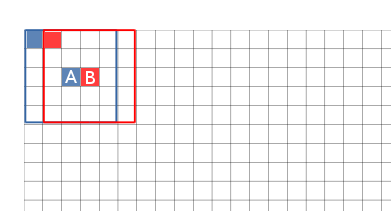
\includegraphics[width=0.5\linewidth]{grid_smooth_colored}
    \caption{Pixels access}
    \label{fig:smoothpa}
\end{figure}
\FloatBarrier

\begin{figure}[!ht]
    \centering
    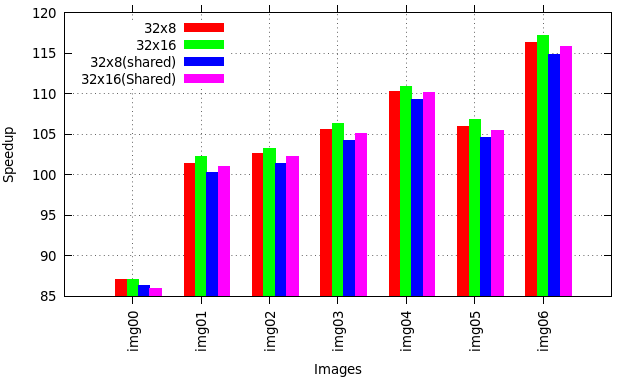
\includegraphics[width=0.7\linewidth]{res/new/smooth_shared_no}
    \caption{Image Portion in Shared Memory VS Global Memory Accesses (different block sizes)}
    \label{fig:smoothsn}
\end{figure}
\FloatBarrier

\subsection{Optimization - More pixels per thread}
\label{sec:sop}
As for the previous algorithms, some additional tests were performed assigning the computation of more pixels per thread. Different thread loads were tested, considering both a dynamic and a fixed grid. Figures \ref{fig:smmo} and \ref{fig:smhf} show the obtained results. With a dynamic approach, varying the number of pixels computed per thread doesn't change a lot the final speedups, except for small images. With a fixed height grid the results are almost the same for every configuration. Figure \ref{fig:smco} shows the comparison of the best dynamic and fixed grid configurations. The results are not so different but the fixed (height) grid approach achieved a little more speedups. For this reason and because it is a more scalable solution, it is the one choosen. Tables \ref{tab:smooth_exe} and \ref{tab:smooth_sp} show the detailed obtained results. Table \ref{tab:smooth_me} shows the total time of the adopted solution, considering also the memory overhead. Table \ref{tab:smooth-abt} exposes the Achieved Throughput and Bandwidth. For the Throughput, for each pixel there are 225 additions, 75 multiplications and 3 divisions. For the Bandwidth, for each pixel there are 75 reads and 3 writes (of 1 byte).
Table \ref{tab:pxabs} shows the differences obtained comparing the output of the sequential algorithm with output of the parallel algorithm.

\begin{figure}[!ht]
    \centering
    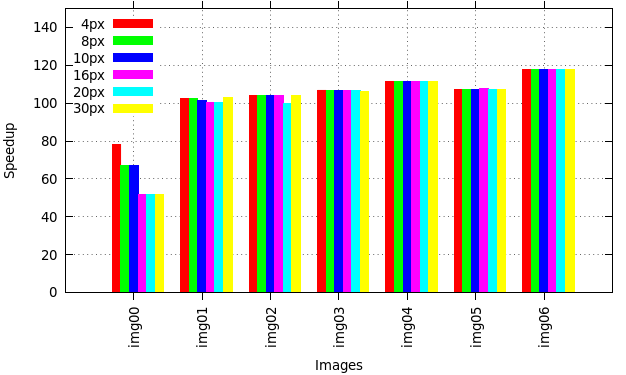
\includegraphics[width=0.7\linewidth]{res/new/smooth_more}
    \caption{More pixels per thread}
    \label{fig:smmo}
\end{figure}
\FloatBarrier

\begin{figure}[!ht]
    \centering
    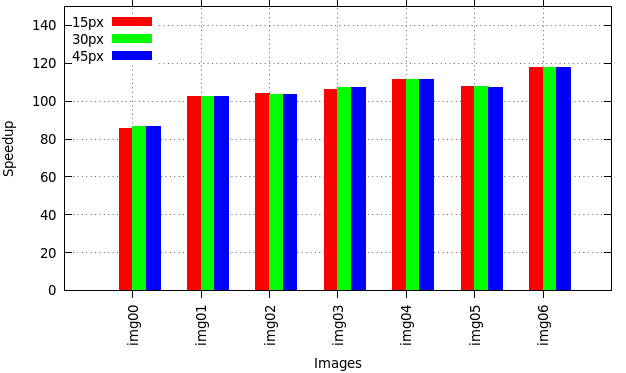
\includegraphics[width=0.7\linewidth]{res/new/smooth_fixed_more}
    \caption{Fixed Height and Dynamic width}
    \label{fig:smhf}
\end{figure}
\FloatBarrier

\begin{figure}[!ht]
    \centering
    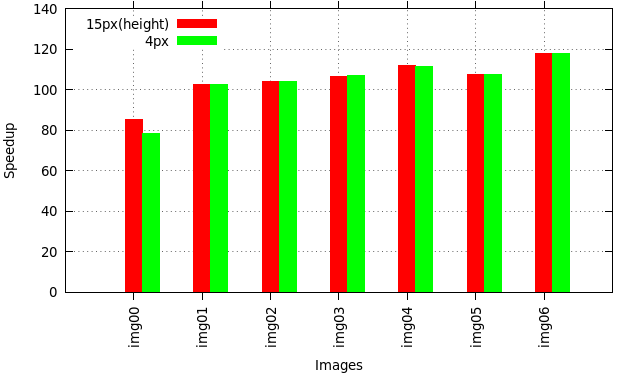
\includegraphics[width=0.7\linewidth]{res/new/smooth_compare}
    \caption{Solutions comparison}
    \label{fig:smco}
\end{figure}
\FloatBarrier

\begin{table}[!ht]
\centering
\begin{tabular}{|l|l|c|c|}
\hline
\textbf{Images} & \textbf{Sequential} & \textbf{15px (height)} & \textbf{4px} \\ \hline
\textbf{Img00}  & 0,067991            & 0,000797               & 0,000868     \\ \hline
\textbf{Img01}  & 0,672104            & 0,006553               & 0,006552     \\ \hline
\textbf{Img02}  & 0,947251            & 0,009093               & 0,009114     \\ \hline
\textbf{Img03}  & 6,496388            & 0,061039               & 0,060738     \\ \hline
\textbf{Img04}  & 4,695295            & 0,042040               & 0,042152     \\ \hline
\textbf{Img05}  & 8,563947            & 0,079630               & 0,079795     \\ \hline
\textbf{Img06}  & 18,571981           & 0,157342               & 0,157640     \\ \hline
\end{tabular}
\caption{Execution Times}
\label{tab:smooth_exe}
\end{table}
\FloatBarrier

\begin{table}[!ht]
\centering
\begin{tabular}{|l|c|c|}
\hline
\textbf{Images} & \textbf{15px (height)} & \textbf{4px} \\ \hline
\textbf{Img00}  & 85,31                  & 78,33        \\ \hline
\textbf{Img01}  & 102,56                 & 102,58       \\ \hline
\textbf{Img02}  & 104,17                 & 103,93       \\ \hline
\textbf{Img03}  & 106,43                 & 106,96       \\ \hline
\textbf{Img04}  & 111,69                 & 111,39       \\ \hline
\textbf{Img05}  & 107,55                 & 107,32       \\ \hline
\textbf{Img06}  & 118,04                 & 117,81       \\ \hline
\end{tabular}
\caption{Speedups}
\label{tab:smooth_sp}
\end{table}
\FloatBarrier



\begin{table}[!ht]
\centering
\begin{tabular}{|l|c|c|c|}
\hline
\textbf{Images} & \textbf{Execution Time (s)} & \textbf{Memory Time(s)} & \textbf{Total(s)} \\ \hline
\textbf{Img00}  & 0,000797                    & 0.000977                & 0.071893          \\ \hline
\textbf{Img01}  & 0,006553                    & 0.006250                & 0.090151          \\ \hline
\textbf{Img02}  & 0,009093                    & 0.009142                & 0.094102          \\ \hline
\textbf{Img03}  & 0,061039                    & 0.057633                & 0.194930          \\ \hline
\textbf{Img04}  & 0,042040                    & 0.038645                & 0.156782          \\ \hline
\textbf{Img05}  & 0,079630                    & 0.061299                & 0.209716          \\ \hline
\textbf{Img06}  & 0,157342                    & 0.147982                & 0.381236          \\ \hline
\end{tabular}
\caption{Measured times}
\label{tab:smooth_me}
\end{table}
\FloatBarrier

\begin{table}[!ht]
\centering
\begin{tabular}{|c|c|c|c|c|}
\hline
\textbf{Images} & \textbf{\begin{tabular}[c]{@{}c@{}}Ach. Throughput\\ (GFLOPS/s)\end{tabular}} & \textbf{\begin{tabular}[c]{@{}c@{}}Ach. Bandwidth\\ (GB/s)\end{tabular}} & \textbf{\begin{tabular}[c]{@{}c@{}}Compute utilization\\ (\%)\end{tabular}} & \textbf{\begin{tabular}[c]{@{}c@{}}Bandwidth utilization\\ (\%)\end{tabular}} \\ \hline
\textbf{Img00}  & 99,66                                                                         & 25,66                                                                    & 7,41                                                                        & 14,46                                                                         \\ \hline
\textbf{Img01}  & 121,21                                                                        & 31,20                                                                    & 9,01                                                                        & 17,59                                                                         \\ \hline
\textbf{Img02}  & 122,84                                                                        & 31,62                                                                    & 9,13                                                                        & 17,83                                                                         \\ \hline
\textbf{Img03}  & 125,30                                                                        & 32,25                                                                    & 9,32                                                                        & 18,18                                                                         \\ \hline
\textbf{Img04}  & 120,92                                                                        & 31,13                                                                    & 8,99                                                                        & 17,55                                                                         \\ \hline
\textbf{Img05}  & 126,11                                                                        & 32,46                                                                    & 9,38                                                                        & 18,30                                                                         \\ \hline
\textbf{Img06}  & 126,21                                                                        & 32,49                                                                    & 9,38                                                                        & 18,31                                                                         \\ \hline
\end{tabular}
\caption{Achieved Throughput and Bandwidth}
\label{tab:smooth-abt}
\end{table}
\FloatBarrier

\begin{table}[!ht]
\centering
\begin{tabular}{|c|l|c|c|l|l|l|l|}
\hline
\textbf{}                        & \textbf{img00}         & \textbf{img01} & \textbf{img02} & \textbf{img03}         & \textbf{img04}         & \textbf{img05}         & \textbf{img06}         \\ \hline
\textbf{Pixels above  threshold} & \multicolumn{1}{c|}{0} & 0              & 0              & \multicolumn{1}{c|}{0} & \multicolumn{1}{c|}{0} & \multicolumn{1}{c|}{0} & \multicolumn{1}{c|}{0} \\ \hline
\end{tabular}
\caption{Differences between the Sequential and the Parallel output}
\label{tab:pxabs}
\end{table}
\FloatBarrier

\newpage

\section{Algorithms analysis with the Visual Profiler}
\label{sec:vp}
After collecting the profile of the applications using \textbf{nvprof} (\textit{prun -v -np 1 -native '-l gpu=GTX480' nvprof --analysis-metrics --output-profile file_name CUDAapp image})
}), the output files were evaluated using the \textbf{Nvidia Visual Profiler} to better understand the applications bottlnecks.

\subsection{Darker}
\label{sec:a1}
 The choosen configuration, uses unidimensional \textit{Blocks} of (1x256) threads, 12 \textit{Registers} and 0 bytes of \textit{Shared Memory}. Table \ref{tab:darker_vp} shows some interesting measurements.
 For all the images the profiler found no issues for \textit{Divergent Execution} (threads that follow different if branches) and a \textit{Warp Execution Efficiency} (ratio of the average active threads per warp to the maximum number of threads per warp supported on a multiprocessor) of 100\%. This last value comes from the fact that is used a block of 256 threads, that is a multiple of 32 (warp size), so no useless threads are launched and from the fact that there is no thread divergent execution, so the threads within a warp can execute in a SIMT way, avoiding inactive threads within the warp. All the the images, obtained an occupancy over 91\% except the first that obtained 80.2\%. This is probably correlated to its small size, but in any case the occupancy is not limiting the performance of the application. For all the images exept the 5th, the Profiler found no issues related to Global Memory Access Pattern. The 5th image, is the only one of the given set that has an amount of pixels that is not a multiple of 128. The memory in the device is allocated with a 128-byte line granularity, so probably, the addresses fall within 2 cache lines when try to read the G and B values and 2 transaction insteads of one are performed (Figure \ref{fig:ucca}). The 2 lines of code in the Listing \ref{div} are the source of the uncoalesced access for \textit{image05}. 
 
 \begin{table}[!ht]
\centering
\begin{tabular}{|c|c|c|c|}
\hline
\textbf{Images} & \textbf{\begin{tabular}[c]{@{}c@{}}Warp Execution Efficiency\\ (\%)\end{tabular}} & \textbf{\begin{tabular}[c]{@{}c@{}}Occupancy\\ (\%)\end{tabular}} & \textbf{\begin{tabular}[c]{@{}c@{}}Branch Divergence\\ (\%)\end{tabular}} \\ \hline
\textbf{Img00}  & 100                                                                               & 80.2                                                              & 0                                                                         \\ \hline
\textbf{Img01}  & 100                                                                               & 91.9                                                              & 0                                                                         \\ \hline
\textbf{Img02}  & 100                                                                               & 92.3                                                              & 0                                                                         \\ \hline
\textbf{Img03}  & 100                                                                               & 93                                                                & 0                                                                         \\ \hline
\textbf{Img04}  & 100                                                                               & 92.5                                                              & 0                                                                         \\ \hline
\textbf{Img05}  & 100                                                                               & 92.3                                                              & 0                                                                         \\ \hline
\textbf{Img06}  & 100                                                                               & 92.8                                                              & 0                                                                         \\ \hline
\end{tabular}
\caption{Visual Profiler Results}
\label{tab:darker_vp}
\end{table}
\FloatBarrier

\begin{figure}[!ht]
 % separation between the subfigures
\begin{subfigure}{0.5\textwidth}
\centering
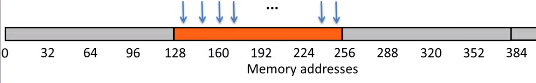
\includegraphics[width=\linewidth]{caching}
\caption{Aligned access}
\label{fig:ca}
\end{subfigure}
 % separation between the subfigures
\begin{subfigure}{0.5\textwidth}
\centering
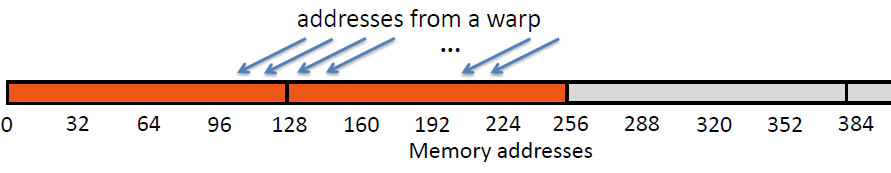
\includegraphics[width=\linewidth]{caching2}
\caption{Unaligned access}
\label{fig:uca}
\end{subfigure}
\caption{Possible access alignements}
 \label{fig:ucca}
\end{figure}
\FloatBarrier

\begin{lstlisting}[label=div, caption=Unaligned accesses]

float g = static_cast< float >(inputImage[(width * height) +
                                          (y * width) + x]);
float b = static_cast< float >(inputImage[(2 * width * height) +
                                          (y * width) + x]);

\end{lstlisting}
\FloatBarrier

\subsection{Histogram}
\label{sec:a2}
The choosen configuration, uses unidimensional \textit{Blocks} of (1x256) threads, 14 \textit{Registers} and 8192 bytes of \textit{Shared Memory}. Table \ref{tab:histo_vp} show some interesting measurements.
For all the images the profiler found issues for \textit{Divergent Execution} and this is due to atomic operations on the shared memory. On the GTX 480, in fact, \_shared\_ memory atomics are implemented not as a single machine instruction, but by a sequence of machine (SASS) instructions that form a loop.
This loop is essentially contending for a lock. When the lock is acquired by a particular thread, that thread will then complete the requested memory operation atomically on the identified shared memory cell, and then release the lock. The process of looping to acquire the lock necessarily involves branch divergence. This problem there would not be using global atomics, that are generally implemented as a single atomic SASS instruction, but as shown before with global atomics worst results were obtained. The profiler, in addition, shows a \textit{Warp Execution Efficiency} that is variable from 50 to 90\%.
This last value comes directly from the fact that there is thread divergent execution, so that some threads within a warp are inactive during the execution. All the images, obtained an occupancy over 91.5\% so the occupancy is not limiting the performance of the application. As for the previous algorithm and for the same reason, for all the images exept the 5th, the Profiler found no issues related to Global Memory Access Pattern. The 2 lines of code that lead to uncoalesced accesses for \textit{image05} are the same as the ones for the previous algorithm (Listing \ref{div2}). For what concerning \textit{bank conflicts}, no optimization can be done, because the accesses to the histograms in shared memory depends on the image.
 

\begin{table}[!ht]
\centering
\begin{tabular}{|c|c|c|c|}
\hline
\textbf{Images} & \textbf{\begin{tabular}[c]{@{}c@{}}Warp Execution Efficiency\\ (\%)\end{tabular}} & \textbf{\begin{tabular}[c]{@{}c@{}}Occupancy\\ (\%)\end{tabular}} & \textbf{\begin{tabular}[c]{@{}c@{}}Branch Divergence\\ (\%)\end{tabular}} \\ \hline
\textbf{Img00}  & 90.7                                                                              & 91.5                                                              & 74.6                                                                      \\ \hline
\textbf{Img01}  & 60.9                                                                              & 98.8                                                              & 93.1                                                                      \\ \hline
\textbf{Img02}  & 52.3                                                                              & 99                                                                & 91.2                                                                      \\ \hline
\textbf{Img03}  & 55.2                                                                              & 99.4                                                              & 90                                                                        \\ \hline
\textbf{Img04}  & 72.5                                                                              & 99.6                                                              & 90                                                                        \\ \hline
\textbf{Img05}  & 64.2                                                                              & 99.4                                                              & 82.2                                                                      \\ \hline
\textbf{Img06}  & 59.5                                                                              & 99.5                                                              & 86.1                                                                      \\ \hline
\end{tabular}
\caption{Visual Profiler Results}
\label{tab:histo_vp}
\end{table}
\FloatBarrier

\subsection{Smooth}
\label{sec:a3}
The choosen configuration, uses bidimensional \textit{Blocks} of (16x32) threads, 21 \textit{Registers} and 0 bytes of \textit{Shared Memory}. Table \ref{tab:smooth_vp} show some interesting measurements. The results seem to be worst than the previous algorithms and there is an explanation. Using 21 registers for each thread, means 10752 registers for each block and this register usage is likely preventing the kernel from fully utilizing the GPU because the \textbf{GTX 480} provide "just" up to 32768 registers for each block. By the way, as suggested by the Profiler the occupacy "is large enough that an increment may not improve performance". The number of registers for the algorithm can't be reduced and testing the same program with smaller blocks the occupancy increased but the overall program obtained worst results as shown before. The explanation is that, if it is possible to achieve fully coalesced accesses to global memory, then a lower occupancy will be sufficient to hide the latency to global memory. As for the previous algorithm and for the same reason, for all the images exept the 5th, the Profiler found no issues related to Global Memory Access Pattern. The 2 lines of code in the Listing \ref{div2} are the source of the uncoalesced access for \textit{image05}.

\begin{table}[!ht]
\centering
\begin{tabular}{|c|c|c|c|}
\hline
\textbf{Images} & \textbf{\begin{tabular}[c]{@{}c@{}}Warp Execution Efficiency\\ (\%)\end{tabular}} & \textbf{\begin{tabular}[c]{@{}c@{}}Occupancy\\ (\%)\end{tabular}} & \textbf{\begin{tabular}[c]{@{}c@{}}Branch Divergence\\ (\%)\end{tabular}} \\ \hline
\textbf{Img00}  & 100                                                                               & 66.1                                                              & 0                                                                         \\ \hline
\textbf{Img01}  & 99.9                                                                              & 66.3                                                              & 3.9                                                                       \\ \hline
\textbf{Img02}  & 99.4                                                                              & 66.3                                                              & 13.8                                                                      \\ \hline
\textbf{Img03}  & 100                                                                               & 66.6                                                              & 0                                                                         \\ \hline
\textbf{Img04}  & 99.6                                                                              & 66.4                                                              & 7.4                                                                       \\ \hline
\textbf{Img05}  & 99.9                                                                              & 66.6                                                              & 0                                                                         \\ \hline
\textbf{Img06}  & 100                                                                               & 66.5                                                              & 0                                                                         \\ \hline
\end{tabular}
\caption{Visual Profiler Results}
\label{tab:smooth_vp}
\end{table}
\FloatBarrier

\begin{lstlisting}[label=div2, caption=Unaligned accesses]
smoothPix += static_cast< float >(inputImage[(z * width * height) + 
                                             (fy * width) + fx]) * 
                                             filter[filterItem];
smoothImage[(z * width * height) + (i * width) + j] = 
                     static_cast< unsigned char >(smoothPix + 0.5f);
\end{lstlisting}
\FloatBarrier

\end{document}

			 	 